\documentclass[11pt]{exam}

\usepackage{amsmath}
\usepackage{graphicx}
\usepackage{geometry}
\usepackage{etoolbox}
\BeforeBeginEnvironment{choices}{\par\nopagebreak\minipage{\linewidth}}
\AfterEndEnvironment{choices}{\endminipage}
\geometry{
a4paper,
total={185mm,257mm},
left=10mm,
top=25mm,
bottom=10mm
}

\begin{document}
\setlength{\voffset}{-0.5in}
\setlength{\headsep}{5pt}

\fbox{\fbox{\parbox{8cm}{\centering
\vspace{2mm}
Testat - Versuch K - Radioaktivitaet 
\vspace{2mm}
}}}
\hspace{2mm}
\makebox[0.25\textwidth]{Name:\enspace\hrulefill} \hspace{5mm}
\makebox[0.2\textwidth]{Datum:\enspace\hrulefill}
\vspace{4mm}

\begin{questions}

\question Die Aktivität einer radioaktiven Substanz wird in Becquerel angegeben. Wie setzt sich diese Größe aus den  SI-Basiseinheiten zusammen?

\begin{choices}
	\choice s
	\choice \( \text{s}^{-1} \)
	\choice \( \text{kg}\cdot\frac{\text{m}}{\text{s}^2} \)
	\choice \( \frac{\text{J}}{\text{kg}} \)
	\choice \( \frac{\text{J}}{\text{s}} \)
\end{choices}

\vspace{3mm}\question Im unten dargestellten Diagramm ist die Aktivität eines radioaktiven Präparates in Abhängigkeit von der Zeit dargestellt. Wie groß ist die Halbwertszeit? 

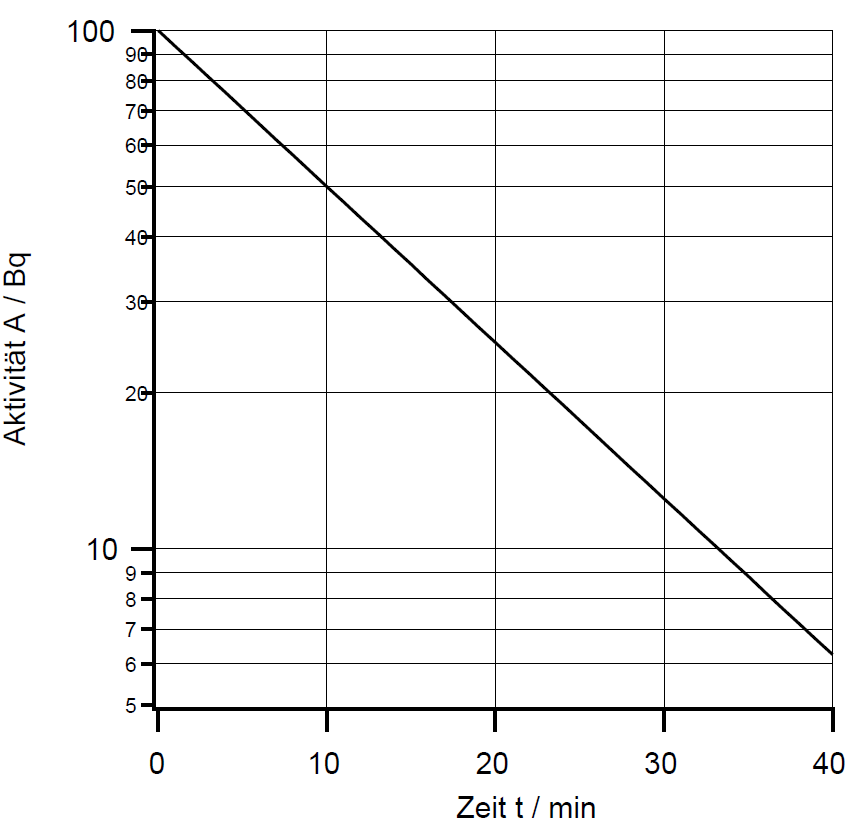
\includegraphics[width=0.4\textwidth]{images/zerfallsgesetz.png}

\begin{choices}
	\choice etwa 100 min
	\choice etwa 5 min
	\choice etwa 10 min
	\choice etwa 20 min
	\choice etwa 1 min
\end{choices}

\vspace{3mm}\question Die Halbwertsdicke eines Absorbers beträgt für radioaktives Barium-137m ca. 5 mm. Wieviel Prozent der Strahlung ist nach 12 mm übrig?

\begin{choices}
	\choice 19 %
	\choice 12,5 %
	\choice 25 %
	\choice 40 %
	\choice 38 %
\end{choices}

\vspace{3mm}\question Welche Aussage ist falsch?

\begin{choices}
	\choice Stoßionisation kommt z.B. in einem Geiger-Müller-Zählrohr vor.
	\choice Elektronen verlieren ihre Energie nur durch Stoßionisationen.
	\choice Gammastrahlung kann z.B. durch den Photoeffekt absorbiert werden.
	\choice Beim Comptoneffekt entsteht Sekundärstrahlung.
	\choice  Beim Photoeffekt entsteht Sekundärstrahlung.
\end{choices}

\vspace{3mm}\question Das Zerfallsgesetz beschreibt den Zusammenhang zwischen der Aktivität einer radioaktiven Quelle und der Zeit. Der Zusammenhang zwischen diesen Größen ist ...

\begin{choices}
	\choice quadratisch.
	\choice exponentiell.
	\choice antiproportional.
	\choice proportional.
	\choice keine der Antworten ist richtig.
\end{choices}

\vspace{3mm}\end{questions}

\end{document}
